\subsection{Beheer van processen en threads in Linux / je kan ook windows of solaris nemen}

\subsubsection{Taken in Linux}

In Linux wordt een proces of taak weergegeven door een task\_struct gegevensstructuur. Deze bevat informatie over een aantal onderwerpen:

















\begin{itemize}
\item Toestand of status v/h proces ( Uitvoering , Gereed , geblokkeerd , opgeschort , zombie ,… )
\item Schedulinginformatie ( informatie nodig om processen in te roosteren )
\item Identificatiecodes: uniek ID per proces + ID voor gebruiker en groep
\item Interprocescommunicatie
\item Verwijzingen ( naar bijvoorbeeld ouder processen of zus-processen )
\item Tijden en klokken ( creatietijdstip + processortijd die al benut is door het proces )
\item Bestandssysteem: verwijzingen naar alle gerelateerde bestanden
\item Adresruimte ( definieert de virtuele adresruimte die toegewezen is aan het proces )
\item Specifieke processorcontext: inhoud van de registers en stack
\end{itemize}

\begin{figure}[htp]
    \centering
            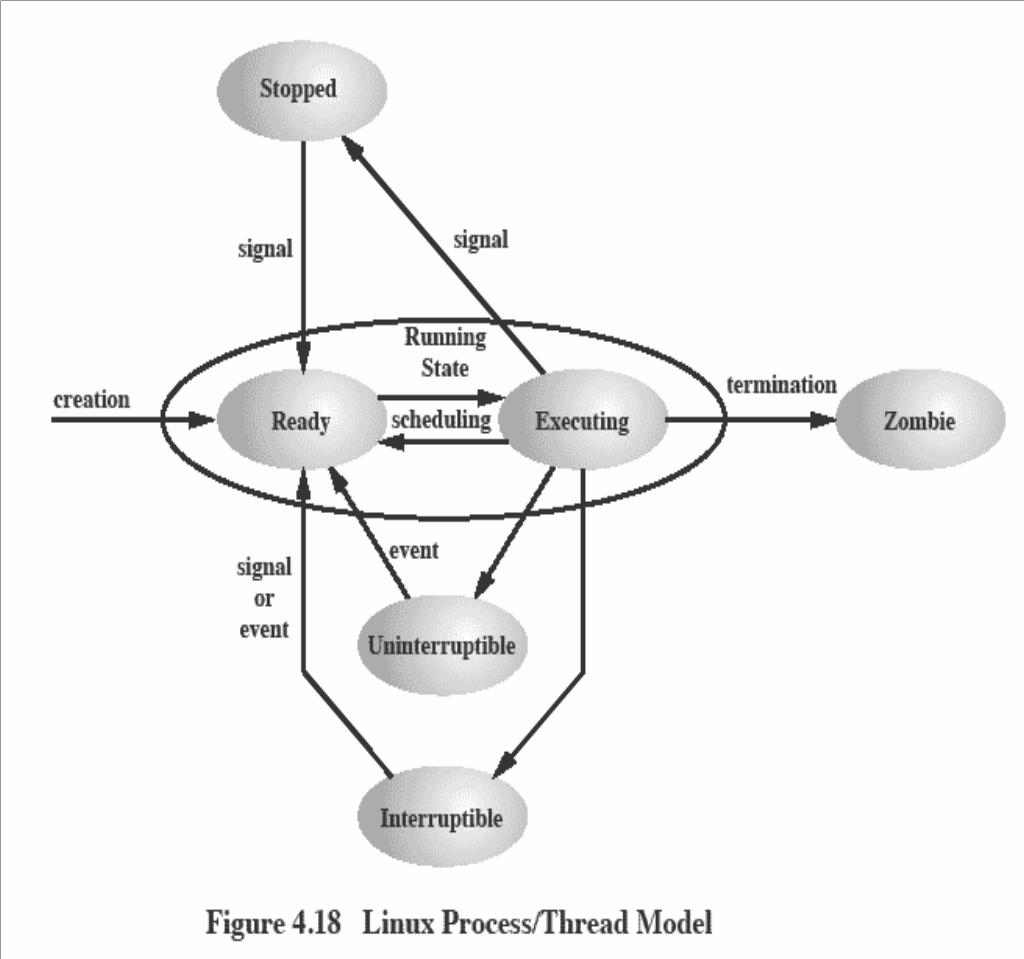
\includegraphics[width=4in]{img/linuxprocessthreadmodel.png}
        \caption{Linux Process/Thread Model}
    \label{fig:Linux Process/Thread Model}
\end{figure}


\newpage


Bovenstaande figuur toont de uitvoeringstoestanden van een proces/thread in Linux:

\begin{itemize}
\item Actief (running): of In Uitvoering, of Gereed.
\item Onderbreekbaar (Interruptable): Het proces wacht op een gebeurtenis
\item Ononderbreekbaar (Uninterruptable): Het proces wacht op een hardwareconditie en zal op niets anders reageren
\item Gestopt (stopped): Het proces is gestopt en kan alleen worden hervat wanneer een ander proces hiervoor actie onderneemt
\item Zombie: Het proces in geëindigd maar beschikt nog wel over zijn taakstructuur in de procestabel
\end{itemize}

\subsubsection{Threads in Linux}

\begin{itemize}
\item Oudere Linux-versies: geen Multithreading.
\item Geen onderscheid tussen threads en processen: threads op gebruikersniveau komen overeen met processen op kernelniveau.
\item Threads van eenzelfde gebruikersproces: zelfde groepsidentificatiecode op kernelniveau.
\item Proces creëren: attributen van huidig proces kopiëren a.h.v. clone().
\item fork() geïmplementeerd a.h.v. clone()
\item Traditionele fork() wordt geïmplementeerd als clone() met alle clone-vlaggen uit
\end{itemize}